% %%%%%%%%%%%%%%%%%%%%%%%%%%%%%%%%%%%%%%%%%%%%%%%%%%%%%%%%%%%%%%%%%%%%%
% %% State-of-the-Art %%
% PHI
% %%%%%%%%%%%%%%%%%%%%%%%%%%%%%%%%%%%%%%%%%%%%%%%%%%%%%%%%%%%%%%%%%%%%%

\subsection{PHI}
\label{sec:soa:phi}

The authors of PHI~\cite{Mukkara2019_PHI} focus on graph algorithms, and include the \acrshort{spmv} kernel as it is core in graph processing.
They note that many large graph algorithms favour pull implementations (each node reads inputs from its neighbours) compared to push implementations (each node propagates results to its neighbours), since in a traditional memory system, push implementations require read-modify-writes which require accessing complete cache-lines, even though a small unit of data is modified.
The push implementation corresponds to the \acrshort{op} algorithm, which suffers from poor memory performance with traditional caches.

PHI is essentially a modified cache which is optimized to efficiently process commutative\footnote{As PHI focuses on graph algorithms, the \gls{reduction} operation could be any commutative operator including logical operations (OR/AND) as well as addition.} \gls{scatter} updates, also called \glspl{reduction}.
It stores, and coalesces values to update, in the cache, as shown in Figures~\ref{fig:soa:phi} and~\ref{fig:soa:phiHow}.
This type of cache is called a \gls{redC}.
PHI works in two phases, managing to take advantage of the two version of the \acrshort{op} algorithm: \textit{immediate updates} and \textit{deferred updates}.
Three new features are introduced, compared to a standard cache:
\begin{itemize}
    \item \textit{In-cache \gls{reduction} storage and processing}.
    In the first phase, when an update for a line not in the cache is received (cache-\gls{miss}), the cache does not fetch the data-line from memory, but rather marks a free cache-line as being in \textit{buffer mode} (\textit{B}), and simply locally stores the update.
    If there are subsequent updates that \gls{hit} the cache-line, they are stored, or combined, using the in-cache commutative operator, as shown in the case~1 of Figure~\ref{fig:soa:phiHow} (top).
    When a cache-line is evicted, if it contains multiple updates, PHI assumes that the coalescing has been effective, and it updates the main memory via a line-wise read-accumulate-write operation.
    This is the normal mode of operation of a traditional \gls{redC}, which processes \textit{immediate updates}.
    %
    \item \textit{Output Batching}.
    In the first phase, if a cache-line is evicted, but contains few updates (managed with a configurable threshold), PHI batches these updates as \textit{(address, value)} tuples, allocating a new cache-line in \textit{update batching mode} (\textit{UB}) to assemble the batch, as shown in the case~2 of Figure~\ref{fig:soa:phiHow} (bottom).
    Groups of updates are organized by \textit{bins} corresponding to a small memory region.
    The batches are streamed to main memory, assembling the \acrfullpl{po} typical of the \textit{deferred updates} \acrshort{op} version.
    Later, in the second phase, the \textit{deferred updates} are read back and processed.
    The reading of the batches is efficient, as they are contiguous (see the \acrshort{op} algorithm in Section~\ref{sec:bg:algos}).
    %
    \item \textit{Reduced Cache Synchronization Traffic}.
    When scaling PHI to multi-core systems, private caches act as local buffers, coalescing the updates and reducing coherency protocol traffic.
\end{itemize}

\begin{figure}[htbp]
    \centering
    \begin{minipage}[b]{0.44545455\linewidth}
        \begin{figure}[H]
            \centering
            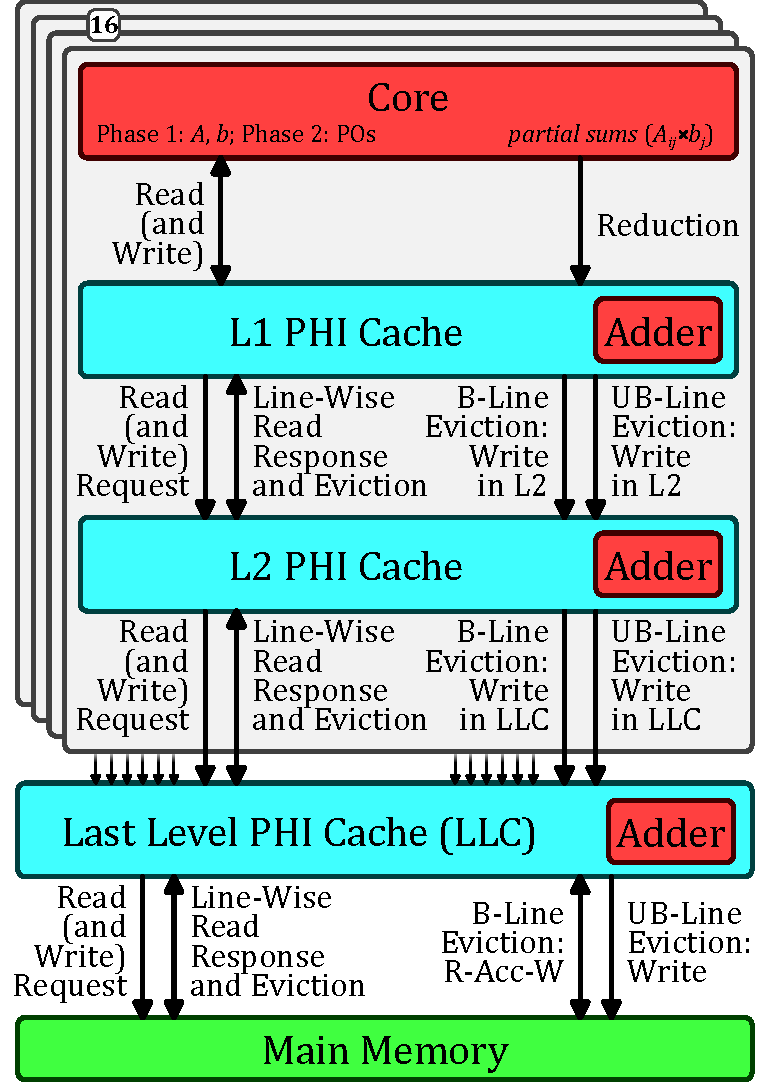
\includegraphics[width=\linewidth]{Chapter_SoA/Figures/PDF/SoA_AcceleratorsArchis_PHI.pdf}
            \caption{Architecture of PHI}
            \label{fig:soa:phi}
        \end{figure}
    \end{minipage}
    \hfill
    \begin{minipage}[b]{0.53636364\linewidth}
        \begin{figure}[H]
            \centering
            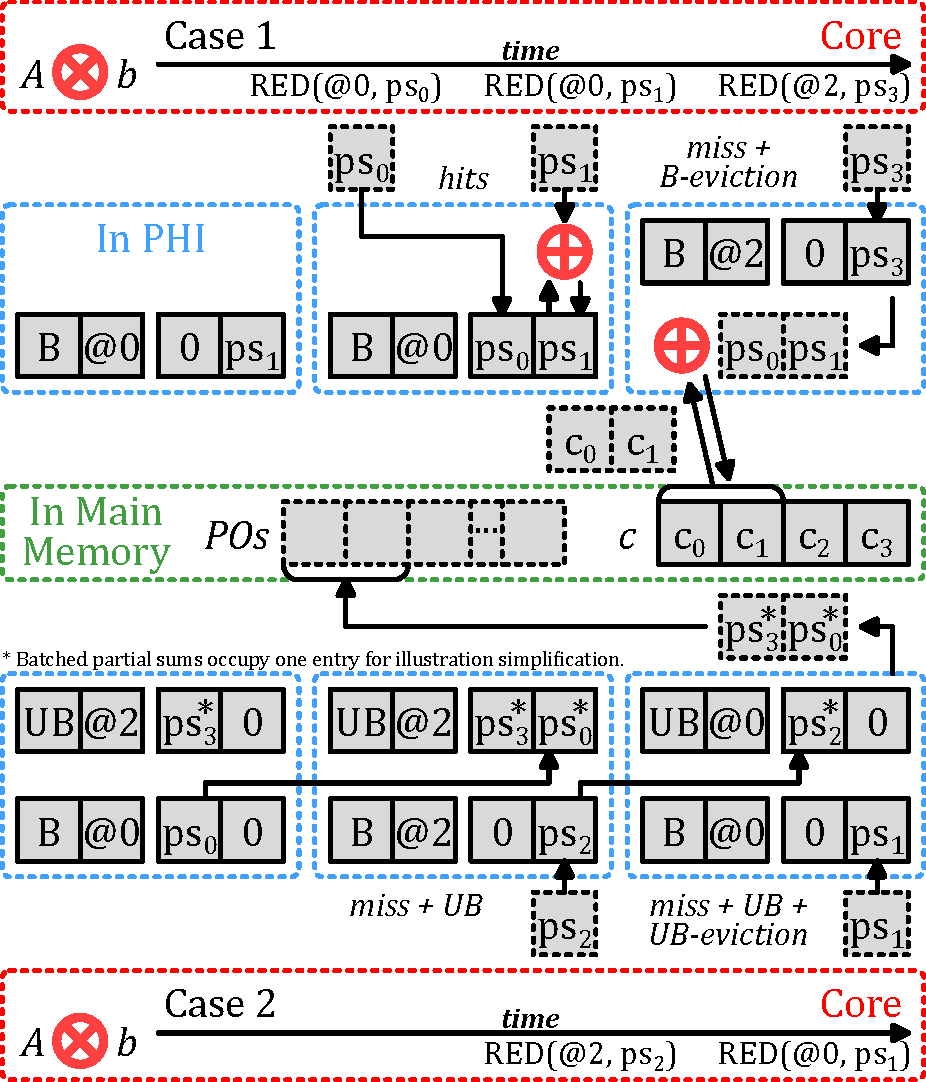
\includegraphics[width=\linewidth]{Chapter_SoA/Figures/PDF/SoA_AcceleratorsArchis_PHI_DF.pdf}
            \caption{PHI Dataflow}
            \label{fig:soa:phiHow}
        \end{figure}
    \end{minipage}
\end{figure}

This combination of in-cache coalescing and update buffering enables PHI to take advantage of locality when possible (like Coup~\cite{Zhang2015_Coup}), but with the addition of \textit{UB}, PHI improves memory utilization, even when the data being updated is too large to fit in the cache.
For \acrshort{spmv}, the authors report that much of the benefit comes from the \gls{reduction} in memory synchronization traffic for multi-core systems.

\begin{highlight}{Conclusion}{Red}
    \textbf{PHI} is a \gls{reduction}-aware cache architecture that optimizes commutative \gls{scatter} updates by combining in-cache coalescing, output batching, and reduced synchronization traffic, effectively improving memory utilization for both \textit{immediate} and \textit{deferred update} \acrshort{op} \acrshort{spmv} kernel.
\end{highlight}